\appendix
\crefalias{section}{appendix}
\crefalias{subsection}{appendix}
\crefalias{subsubsection}{appendix}
\section{Appendices}
\subsection{SDS Information} % This will be Appendix A
\label{app:SDS}

\begin{tabular}{p{0.18\linewidth}p{0.3\linewidth}p{0.5\linewidth}}
\toprule
Chemical & Hazards & Treatments \\
\midrule
Acetone & Flammable in both its liquid and vapor forms, may cause irritation of respiratory tract, vapors may cause drowsiness, and repeated exposure may cause skin dryness. & Rinse eyes immediately upon contact, wash skin immediately upon contact, move to fresh air if inhaled, and obtain medical attention if ingested. \\ \\
Hydrochloric acid & Corrosive to metals, may cause skin corrosion/irritation, eye damage/irritation, and respiratory system toxicity. & Rinse eyes immediately upon contact, wash skin immediately upon contact, call Poison Center Control if ingested, and move to fresh air if inhaled. \\ \\
Hydrogen iodide & Corrosive to the respiratory system, eyes, and skin, harmful/toxic if inhaled, and causes burns. & Rinse eyes immediately upon contact, wash skin immediately upon contact, move to fresh air if inhaled, wash out mouth with water and seek medical attention if ingested. \\ \\
Iodine water & Irritating to skin and body tissues. & Rinse eyes immediately upon contact, wash skin immediately upon contact, move to fresh air if inhaled, and rinse out mouth with water or milk, induce vomiting, and seek medical attention if ingested. \\
\bottomrule
\end{tabular}
\subsubsection*{SDS references}
\begin{enumerate}
    \item Fisher Scientific. Acetone Material Safety Data Sheet. 2009. \url{https://udel.instructure.com/courses/1903743/files/folder/KIN%20Resources/2025/1.%20MSDS?preview=156346371}

    \item Fisher Scientific. Hydrochloric Acid Material Safety Data Sheet. 2009. \url{https://udel.instructure.com/courses/1903743/files/folder/KIN%20Resources/2025/1.%20MSDS?preview=156346373}

    \item ThermoFisher Scientific. Hydrochloric Acid Safety Data Sheet. 2009. \url{https://www.fishersci.com/store/msds?partNumber=A481212&productDescription=HYDROCHLORIC+ACID+NF%2FFCC+21%2F2L&vendorId=VN00033897&countryCode=US&language=en}

    \item Fisher Scientific. Hydrogen Iodide Material Safety Data Sheet. 2009. \url{https://udel.instructure.com/courses/1903743/files/folder/KIN%20Resources/2025/1.%20MSDS?preview=156346372}

    \item Flinn Scientific Inc. Iodine Water Material Safety Data Sheet. 2002. \url{https://udel.instructure.com/courses/1903743/files/folder/KIN%20Resources/2025/1.%20MSDS?preview=156346380}
\end{enumerate}



\subsection{Data Processing}
\label{app:processing}

Each individual signal was processed through the following pipeline
\begin{enumerate}
    \item The absorbance values in the signal were converted to concentration values using the calibration curve for the UV-vis spectrophotometer used to collect the signal.
    \item From there, outliers were removed from the signal using random sample consensus RANSAC \autocite{RANSAC} as the outliers are “gross” meaning the significant outliers are strictly greater than the mean and not normally distributed about the mean.
    \item A loss function of absolute error was used and considered points with a residual greater than 0.00001 M as outliers.
    \item A line was then fit to the concentration data and the slope saved as the reaction rate. 
\end{enumerate}
To obtain temperature for each reaction, the start time of the reaction was noted. For a reaction with n absorbance measurements, n temperature measurements were considered after the noted start time when calculating the average and standard deviation. An illustration of outlier removal with RANSAC is shared below.

\begin{figure}[H]
    \centering
    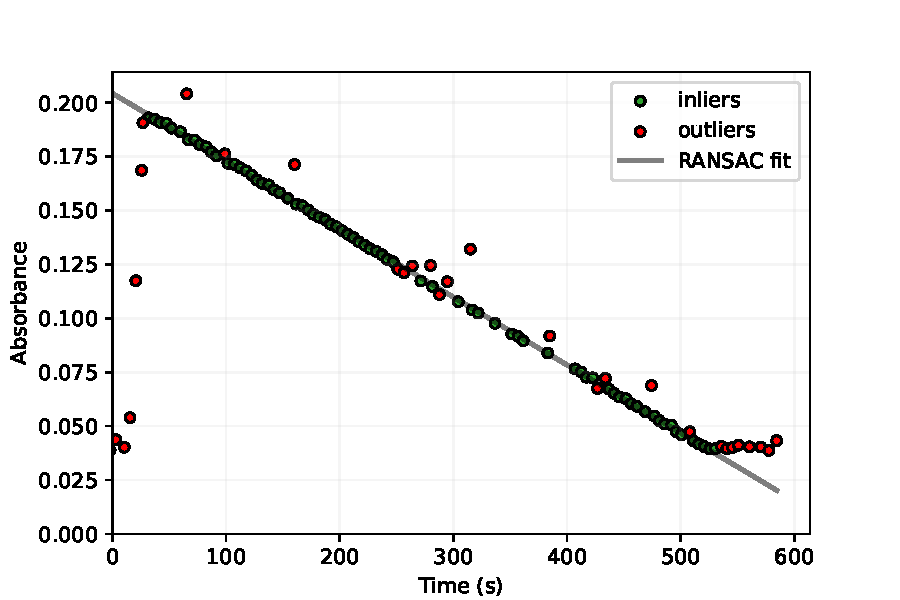
\includegraphics[width=0.8\linewidth]{figures/RANSAC.pdf}
    \caption{Illustrative RANSAC outlier detection. The red points have been identified as outliers and it should be noted that the outliers are almost strictly above the mean as opposed to being distributed normally around the mean.}
    \label{fig:ransac}
\end{figure}



\subsection{Reaction Order Data}
\label{app:orderData}
This data is additionally available for download on Github \url{https://github.com/kylecapybara/cheg345kin}.

\begin{table}[H]
\centering
\caption{Experimental data for iodination of acetone under varying conditions.}

\begin{subtable}{\textwidth}
\centering
\caption{Collected data for determining reaction order with respect to hydrochloric acid.}
\begin{tabular}{rrrrr}
\toprule
Temperature (ºC) & [HCl] (M) & [I$_2$] (M) & [Acetone] (M) & Rate (M/s) \\
\midrule
2.956e+01 & 2.411e-02 & 2.130e-03 & 1.990e+00 & 4.700e-06 \\
2.941e+01 & 1.134e-02 & 2.290e-03 & 1.980e+00 & 2.170e-06 \\
2.936e+01 & 4.082e-02 & 2.000e-03 & 1.970e+00 & 7.570e-06 \\
\bottomrule
\end{tabular}
\end{subtable}

\vspace{0.75em}

\begin{subtable}{\textwidth}
\centering
\caption{Collected data for determining reaction order with respect to iodine}
\begin{tabular}{rrrrr}
\toprule
Temperature (ºC) & [HCl] (M) & [I$_2$] (M) & [Acetone] (M) & Rate (M/s) \\
\midrule
2.956e+01 & 2.411e-02 & 2.130e-03 & 1.990e+00 & 4.700e-06 \\
2.927e+01 & 2.054e-02 & 4.180e-03 & 1.950e+00 & 3.570e-06 \\
2.956e+01 & 2.094e-02 & 1.030e-03 & 1.990e+00 & 4.460e-06 \\
\bottomrule
\end{tabular}
\end{subtable}

\vspace{0.75em}

\begin{subtable}{\textwidth}
\centering
\caption{Collected data for determining reaction order with respect to acetone}
\begin{tabular}{rrrrr}
\toprule
Temperature (ºC) & [HCl] (M) & [I$_2$] (M) & [Acetone] (M) & Rate (M/s) \\
\midrule
2.956e+01 & 2.411e-02 & 2.130e-03 & 1.990e+00 & 4.700e-06 \\
2.927e+01 & 2.009e-02 & 3.010e-03 & 4.660e-01 & 7.330e-07 \\
2.974e+01 & 2.069e-02 & 2.150e-03 & 4.030e+00 & 8.210e-06 \\
\bottomrule
\end{tabular}
\end{subtable}

\end{table}




\subsection{Collected Signals}
\label{app:signals}

\cref{fig:collectedsignals} shares all of collected signals with outliers removed and the peak absorbance set to a time of zero seconds. 

\begin{figure}[H]
    \centering
    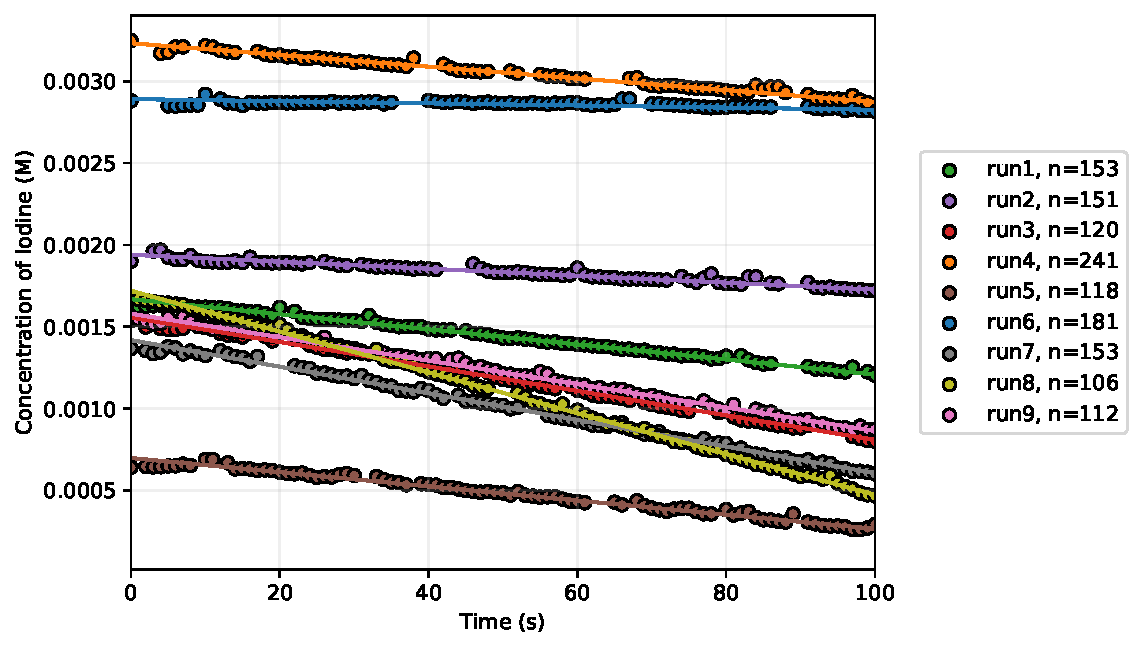
\includegraphics[width=0.75\linewidth]{figures/collecteddata.pdf}
    \caption{Collected signals with outliers removed and linear fits.}
    \label{fig:collectedsignals}
\end{figure}

These collected signals were converted from absorbance to concentrating using the following calibration curves as provided by the instructional team. The provided calibration curves are shared below in \cref{fig:calibrationcurve}.

\begin{figure}[H]
    \centering
    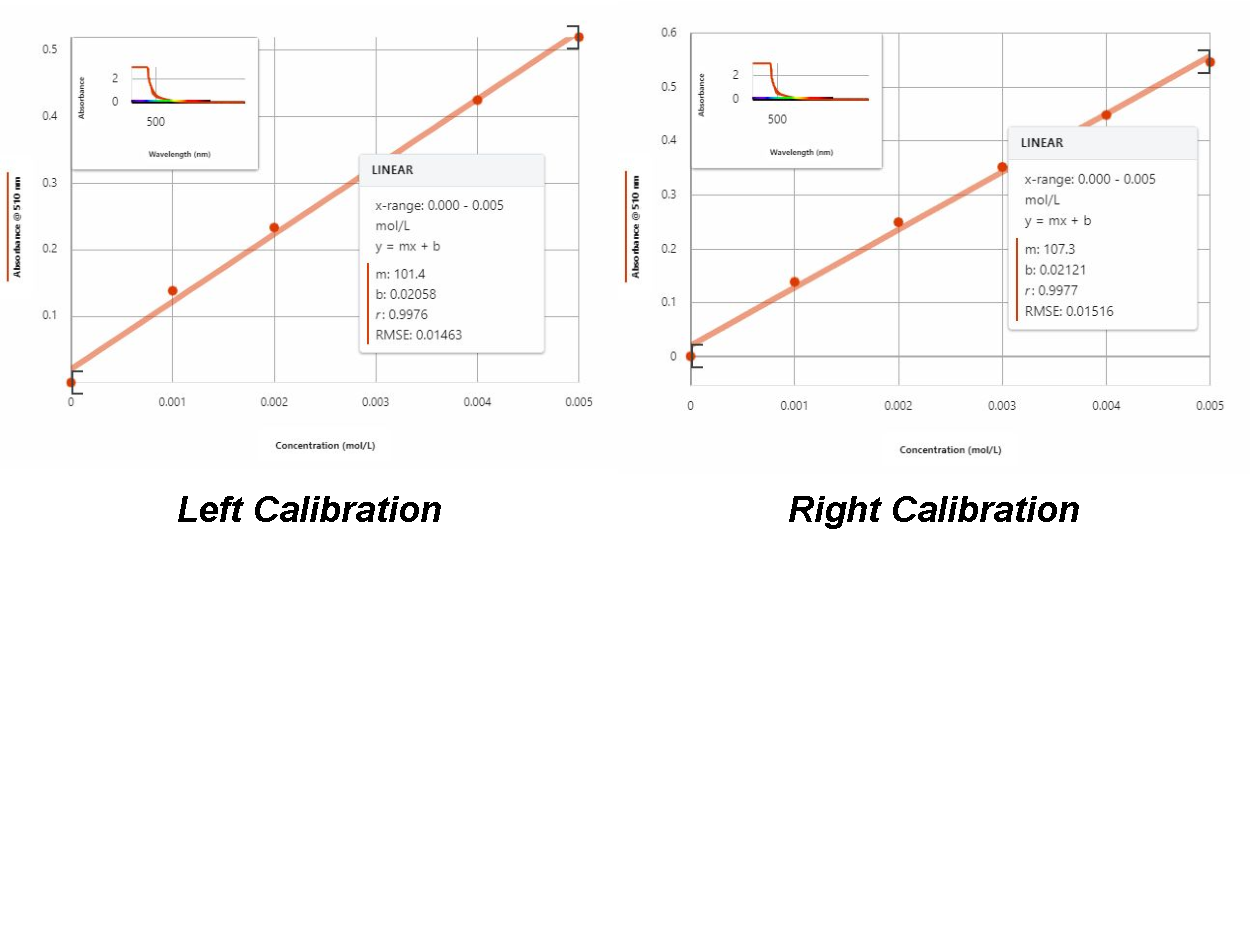
\includegraphics[width=0.9\linewidth]{figures/calibration.pdf}
    \caption{Calibration curves relating iodine concentration to absorbance.}
    \label{fig:calibrationcurve}
\end{figure}


\subsection{Propagation of Uncertainty}
\label{app:errorProp}

Rearranging the linearized rate law arrives at equation \cref{eq:lnk},

\begin{equation}
    \ln(k) = \ln(\mathrm{Rate}) - \alpha \ln([\mathrm{Ac}]) - \beta \ln([\mathrm{H_3O^+}]) - \gamma \ln([\mathrm{I_2}])
    \label{eq:lnk}
\end{equation}

Treating the uncertainties in concentration as negligible, the uncertainty in $\ln(k)$ arises from the uncertainties in the fitted exponents $\alpha$, $\beta$, $\gamma$, and in the measured rate. Applying standard propagation of uncertainty to \cref{eq:lnk}:

\begin{equation}
    \delta \ {\ln(k)} = \sqrt{
        \left(\frac{\partial \ln(k)}{\partial \ln(\mathrm{Rate})}\,\delta \ {\ln(\mathrm{Rate})}\right)^2
      + \left(\frac{\partial \ln(k)}{\partial \alpha}\,\delta\alpha\right)^2
      + \left(\frac{\partial \ln(k)}{\partial \beta}\,\delta\beta\right)^2
      + \left(\frac{\partial \ln(k)}{\partial \gamma}\,\delta\gamma\right)^2
    }
\end{equation}
Evaluating each partial derivative from \cref{eq:lnk},

\begin{align*}
    \frac{\partial \ln(k)}{\partial \ln(\mathrm{Rate})} &= 1 \\[4pt]
    \frac{\partial \ln(k)}{\partial \alpha} &= -\ln([\mathrm{Ac}]) \\[4pt]
    \frac{\partial \ln(k)}{\partial \beta}  &= -\ln([\mathrm{H_3O^+}]) \\[4pt]
    \frac{\partial \ln(k)}{\partial \gamma} &= -\ln([\mathrm{I_2}])
\end{align*}
Substituting,

\begin{equation}
    \delta \ {\ln(k)} = \sqrt{
        \left(\delta \ {\ln(\mathrm{Rate})}\right)^2
      + \bigl(\ln([\mathrm{Ac}])\,\delta\alpha\bigr)^2
      + \bigl(\ln([\mathrm{H_3O^+}])\,\delta\beta\bigr)^2
      + \bigl(\ln([\mathrm{I_2}])\,\delta\gamma\bigr)^2
    }
    \label{eq:pou_lnk1}
\end{equation}
The uncertainty in $\ln(\mathrm{Rate})$ is obtained by propagating $\delta\mathrm{Rate}$ through the logarithm:
\begin{equation*}
    \delta\ln(\mathrm{Rate}) = \left|\frac{d\ln(\mathrm{Rate})}{d\,\mathrm{Rate}}\right| \delta\mathrm{Rate} = \frac{\delta\mathrm{Rate}}{\mathrm{Rate}}
\end{equation*}
Substituting this result into \cref{eq:pou_lnk1} yields the following (as presented earlier in the body of this report).
\begin{equation}
    \delta \ {\ln(k)} = \sqrt{
        \left( {\frac{\delta\mathrm{Rate}}{\mathrm{Rate}}}\right)^2
      + \bigl(\ln([\mathrm{Ac}])\,\delta\alpha\bigr)^2
      + \bigl(\ln([\mathrm{H_3O^+}])\,\delta\beta\bigr)^2
      + \bigl(\ln([\mathrm{I_2}])\,\delta\gamma\bigr)^2
    }
    \label{eq:pou_lnk2}
\end{equation}
It should be noted that a formula derived not neglecting the contributions from the error in the concentrations was tested and produced error bars indistinguishable from the result neglecting the error in concentrations.

\subsection{Statistical Tests}
\label{app:tests}

All tests were two-tailed $t$-tests implemented using \texttt{scipy.stats.t}.

\subsubsection*{Hypothesis Framework}

For each parameter $\theta$ with estimated value $\hat{\theta}$ and standard error $s_{\hat{\theta}}$,
the null hypothesis is that the parameter equals the theoretical or literature value $\theta_0$:
\begin{equation}
    H_0: \theta = \theta_0 \qquad H_a: \theta \neq \theta_0
\end{equation}
The t-statistic is then
\begin{equation}
    t = \frac{\hat{\theta} - \theta_0}{s_{\hat{\theta}}}
\end{equation}
where the standard error is estimated from the sample standard deviation, $\sigma$, of the estimated parameter values across the $N$ repeated measurements,
\begin{equation}
    s_{\hat{\theta}} = \frac{\sigma}{\sqrt{N}}
\end{equation}
P-values were computed from the two-tailed cumulative distribution function of the $t$-distribution at $\nu = N - n$ degrees of freedom where $N$ is the number of collected data points and $n$ is the number of fit model parameters.

\subsubsection*{Reaction Orders}

Reaction orders were tested against the theoretical values predicted by the pseudo-equilibrium mechanism: $\alpha_0 = 1$, $\beta_0 = 1$, $\gamma_0 = 0$. For each species, three repeated measurements were collected at varying concentration of that species while holding all others fixed, giving $N = 3$ and $\nu = 1$ degrees of freedom. 

\subsubsection*{Activation Energy}

The experimentally determined activation energy was compared against the literature value reported by Albery and Robinson \cite{albery_measurement_1969} of $E_{a,\mathrm{lit}} = 86.60\ \mathrm{kJ\ mol^{-1}}$. The literature value is treated as a known population parameter. Rate constants were computed at each of the three experimental temperatures, giving $N = 3$ and $\nu = 1$ degrees of freedom. The standard error of $\hat{E}_a$ is therefore \cref{eq:seEa} where $\sigma_m$ is the standard error of the slope of the regression line which comes from the square root of the diagonal entries of the covariance matrix.
\begin{equation}
    s_{\hat{E}_a} = - R \,\cdot \sigma_m \label{eq:seEa}
\end{equation}
The test statistic is then,
\begin{equation}
    t = \frac{\hat{E}_a - E_{a,\mathrm{lit}}}{s_{\hat{E}_a}}
    = \frac{(111{,}200 - 86{,}600)\ \mathrm{J\ mol^{-1}}}{s_{\hat{E}_a}}.
\end{equation}
This yields $t = 4.98$ at $\nu = 1$, giving $p = 0.126$, indicating  statistical agreement with the literature consensus. 

\subsection{Plotting Confidence Intervals}
\label{app:plotCI}
To generate 95\% confidence interval on plots with linear regression the following equations were used.

\[
x_i=\frac{1}{T_i},\qquad y_i=\ln(k_i),\qquad \hat y(x)=\hat\beta_0+\hat\beta_1 x
\]
\[
s=\sqrt{\frac{\sum_{i=1}^{n}(y_i-\hat y_i)^2}{n-2}},\qquad
S_{xx}=\sum_{i=1}^{n}(x_i-\bar x)^2
\]
From these equations, the 95\% CI upper and lower bounds are given by $\hat{y}_{x_0}$ as shared in \cref{eq:CIlines}.
\begin{equation}
    \hat y(x)\pm t_{0.975,\;n-2}\,s\sqrt{\frac{1}{n}+\frac{(x-\bar x)^2}{S_{xx}}} \label{eq:CIlines}
\end{equation}

\subsection{Pressure Rack Data}
\label{app:pressure}

\begin{table}[H]
    \centering
    \caption{Pressures in First Flow Line}
    \label{tab:firstflowline}
    \begin{tabular}{lccccc}
        \toprule
        & P1 & P2 & P3 & P4 & P5 \\
        \midrule
        Bourdon Gauge (psi)        & 10.0 & 11.0 & 16.5 & 19.0 & 20.0 \\
        Digital Gauge (MPa)        & 0.139 & 0.179 & 0.206 & 0.243 & 0.280 \\
        Other Bourdon Gauge (psi)  & 20.0 & 26.0 & 30.0 & 35.0 & 40.1 \\
        Uncertainty                & 0.1 & 0.1 & 0.1 & 0.1 & 0.1 \\
        \bottomrule
    \end{tabular}
\end{table}

% Requires: \usepackage{booktabs}
\begin{table}[H]
    \centering
    \caption{Pressures in Second Flow Line}
    \label{tab:secondflowline}
    \begin{tabular}{lccccc}
        \toprule
        2nd Line & P1 & P2 & P3 & P4 & P5 \\
        \midrule
        Rotameter     & 1000 & 800 & 600 & 400 & 200 \\
        MFC Set Point & 0.932 & 0.739 & 0.572 & 0.389 & 0.203 \\
        \bottomrule
    \end{tabular}
\end{table}

\begin{table}[H]
    \centering
    \caption{Pressures in Third Flow Line}
    \label{tab:thirdflowline}
    \begin{tabular}{lccccc}
        \toprule
        3rd Line & P1 & P2 & P3 & P4 & P5 \\
        \midrule
        Bourdon Gauge & 19.5 & 25.0 & 30.0 & 35.0 & 40.0 \\
        Transducer    & 20.06 & 26.26 & 31.26 & 35.70 & 40.56 \\
        \bottomrule
    \end{tabular}
\end{table}

\begin{table}[H]
    \centering
    \caption{Pressure \& Electric Signal in Fourth Flow Line}
    \label{tab:fourthflowline}
    \begin{tabular}{ll}
        \toprule
        4th Line                &  \\ \midrule
        Pressure & 15 psi \\
        Pneumatic Valve (psi)   & 16.2 \\
        EM Transducer (V)       & 4.4 \\
        \bottomrule
    \end{tabular}
\end{table}



\subsection{Numerical Simulation of BSTR}
\label{app:bstr}

The python code used to model the autocatalytic behavior in a BSTR is available on Github (\url{https://github.com/kylecapybara/cheg345kin/blob/main/bstr/bstr_UPDATED.ipynb})

\subsection{CSTR Sizing}

The python code used for CSTR sizing and sensitivity analysis is available on Github (\url{https://github.com/kylecapybara/cheg345kin/blob/main/cstrsizing.py})


